% Created by tikzDevice version 0.12 on 2019-02-01 11:55:22
% !TEX encoding = UTF-8 Unicode
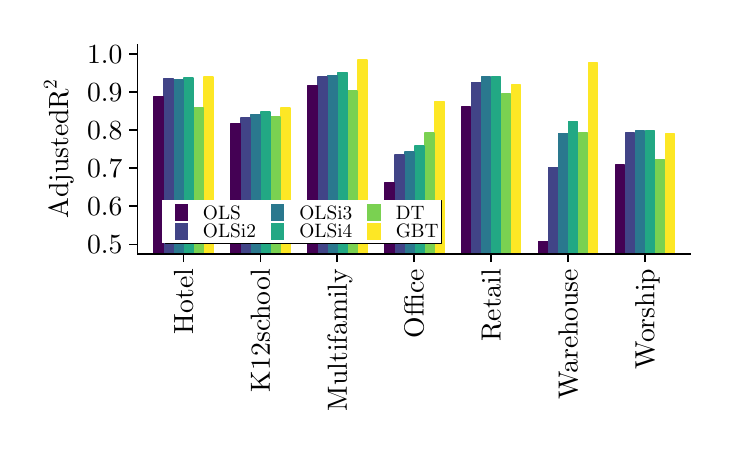
\begin{tikzpicture}[x=1pt,y=1pt]
\definecolor{fillColor}{RGB}{255,255,255}
\path[use as bounding box,fill=fillColor,fill opacity=0.00] (0,0) rectangle (245.72,144.54);
\begin{scope}
\path[clip] (  0.00,  0.00) rectangle (245.72,144.54);
\definecolor{drawColor}{RGB}{255,255,255}
\definecolor{fillColor}{RGB}{255,255,255}

\path[draw=drawColor,line width= 0.6pt,line join=round,line cap=round,fill=fillColor] (  0.00,  0.00) rectangle (245.72,144.54);
\end{scope}
\begin{scope}
\path[clip] ( 39.64, 62.78) rectangle (239.72,138.54);
\definecolor{fillColor}{RGB}{255,255,255}

\path[fill=fillColor] ( 39.64, 62.78) rectangle (239.72,138.54);
\definecolor{drawColor}{RGB}{253,231,37}
\definecolor{fillColor}{RGB}{253,231,37}

\path[draw=drawColor,line width= 0.6pt,line join=round,fill=fillColor] ( 63.73, -2.66) rectangle ( 66.97,126.83);
\definecolor{drawColor}{RGB}{122,209,81}
\definecolor{fillColor}{RGB}{122,209,81}

\path[draw=drawColor,line width= 0.6pt,line join=round,fill=fillColor] ( 60.11, -2.66) rectangle ( 63.36,115.67);
\definecolor{drawColor}{RGB}{34,168,132}
\definecolor{fillColor}{RGB}{34,168,132}

\path[draw=drawColor,line width= 0.6pt,line join=round,fill=fillColor] ( 56.50, -2.66) rectangle ( 59.74,126.42);
\definecolor{drawColor}{RGB}{42,120,142}
\definecolor{fillColor}{RGB}{42,120,142}

\path[draw=drawColor,line width= 0.6pt,line join=round,fill=fillColor] ( 52.89, -2.66) rectangle ( 56.13,125.59);
\definecolor{drawColor}{RGB}{65,68,135}
\definecolor{fillColor}{RGB}{65,68,135}

\path[draw=drawColor,line width= 0.6pt,line join=round,fill=fillColor] ( 49.28, -2.66) rectangle ( 52.52,126.14);
\definecolor{drawColor}{RGB}{68,1,84}
\definecolor{fillColor}{RGB}{68,1,84}

\path[draw=drawColor,line width= 0.6pt,line join=round,fill=fillColor] ( 45.66, -2.66) rectangle ( 48.91,119.67);
\definecolor{drawColor}{RGB}{253,231,37}
\definecolor{fillColor}{RGB}{253,231,37}

\path[draw=drawColor,line width= 0.6pt,line join=round,fill=fillColor] ( 91.51, -2.66) rectangle ( 94.76,115.40);
\definecolor{drawColor}{RGB}{122,209,81}
\definecolor{fillColor}{RGB}{122,209,81}

\path[draw=drawColor,line width= 0.6pt,line join=round,fill=fillColor] ( 87.90, -2.66) rectangle ( 91.14,112.23);
\definecolor{drawColor}{RGB}{34,168,132}
\definecolor{fillColor}{RGB}{34,168,132}

\path[draw=drawColor,line width= 0.6pt,line join=round,fill=fillColor] ( 84.29, -2.66) rectangle ( 87.53,114.02);
\definecolor{drawColor}{RGB}{42,120,142}
\definecolor{fillColor}{RGB}{42,120,142}

\path[draw=drawColor,line width= 0.6pt,line join=round,fill=fillColor] ( 80.68, -2.66) rectangle ( 83.92,113.19);
\definecolor{drawColor}{RGB}{65,68,135}
\definecolor{fillColor}{RGB}{65,68,135}

\path[draw=drawColor,line width= 0.6pt,line join=round,fill=fillColor] ( 77.06, -2.66) rectangle ( 80.31,111.82);
\definecolor{drawColor}{RGB}{68,1,84}
\definecolor{fillColor}{RGB}{68,1,84}

\path[draw=drawColor,line width= 0.6pt,line join=round,fill=fillColor] ( 73.45, -2.66) rectangle ( 76.69,109.89);
\definecolor{drawColor}{RGB}{253,231,37}
\definecolor{fillColor}{RGB}{253,231,37}

\path[draw=drawColor,line width= 0.6pt,line join=round,fill=fillColor] (119.30, -2.66) rectangle (122.54,132.89);
\definecolor{drawColor}{RGB}{122,209,81}
\definecolor{fillColor}{RGB}{122,209,81}

\path[draw=drawColor,line width= 0.6pt,line join=round,fill=fillColor] (115.69, -2.66) rectangle (118.93,121.73);
\definecolor{drawColor}{RGB}{34,168,132}
\definecolor{fillColor}{RGB}{34,168,132}

\path[draw=drawColor,line width= 0.6pt,line join=round,fill=fillColor] (112.08, -2.66) rectangle (115.32,128.35);
\definecolor{drawColor}{RGB}{42,120,142}
\definecolor{fillColor}{RGB}{42,120,142}

\path[draw=drawColor,line width= 0.6pt,line join=round,fill=fillColor] (108.46, -2.66) rectangle (111.71,127.24);
\definecolor{drawColor}{RGB}{65,68,135}
\definecolor{fillColor}{RGB}{65,68,135}

\path[draw=drawColor,line width= 0.6pt,line join=round,fill=fillColor] (104.85, -2.66) rectangle (108.09,126.83);
\definecolor{drawColor}{RGB}{68,1,84}
\definecolor{fillColor}{RGB}{68,1,84}

\path[draw=drawColor,line width= 0.6pt,line join=round,fill=fillColor] (101.24, -2.66) rectangle (104.48,123.66);
\definecolor{drawColor}{RGB}{253,231,37}
\definecolor{fillColor}{RGB}{253,231,37}

\path[draw=drawColor,line width= 0.6pt,line join=round,fill=fillColor] (147.09, -2.66) rectangle (150.33,117.88);
\definecolor{drawColor}{RGB}{122,209,81}
\definecolor{fillColor}{RGB}{122,209,81}

\path[draw=drawColor,line width= 0.6pt,line join=round,fill=fillColor] (143.48, -2.66) rectangle (146.72,106.44);
\definecolor{drawColor}{RGB}{34,168,132}
\definecolor{fillColor}{RGB}{34,168,132}

\path[draw=drawColor,line width= 0.6pt,line join=round,fill=fillColor] (139.87, -2.66) rectangle (143.11,101.76);
\definecolor{drawColor}{RGB}{42,120,142}
\definecolor{fillColor}{RGB}{42,120,142}

\path[draw=drawColor,line width= 0.6pt,line join=round,fill=fillColor] (136.25, -2.66) rectangle (139.49, 99.56);
\definecolor{drawColor}{RGB}{65,68,135}
\definecolor{fillColor}{RGB}{65,68,135}

\path[draw=drawColor,line width= 0.6pt,line join=round,fill=fillColor] (132.64, -2.66) rectangle (135.88, 98.59);
\definecolor{drawColor}{RGB}{68,1,84}
\definecolor{fillColor}{RGB}{68,1,84}

\path[draw=drawColor,line width= 0.6pt,line join=round,fill=fillColor] (129.03, -2.66) rectangle (132.27, 88.54);
\definecolor{drawColor}{RGB}{253,231,37}
\definecolor{fillColor}{RGB}{253,231,37}

\path[draw=drawColor,line width= 0.6pt,line join=round,fill=fillColor] (174.88, -2.66) rectangle (178.12,123.80);
\definecolor{drawColor}{RGB}{122,209,81}
\definecolor{fillColor}{RGB}{122,209,81}

\path[draw=drawColor,line width= 0.6pt,line join=round,fill=fillColor] (171.27, -2.66) rectangle (174.51,120.49);
\definecolor{drawColor}{RGB}{34,168,132}
\definecolor{fillColor}{RGB}{34,168,132}

\path[draw=drawColor,line width= 0.6pt,line join=round,fill=fillColor] (167.65, -2.66) rectangle (170.90,126.83);
\definecolor{drawColor}{RGB}{42,120,142}
\definecolor{fillColor}{RGB}{42,120,142}

\path[draw=drawColor,line width= 0.6pt,line join=round,fill=fillColor] (164.04, -2.66) rectangle (167.28,126.69);
\definecolor{drawColor}{RGB}{65,68,135}
\definecolor{fillColor}{RGB}{65,68,135}

\path[draw=drawColor,line width= 0.6pt,line join=round,fill=fillColor] (160.43, -2.66) rectangle (163.67,124.76);
\definecolor{drawColor}{RGB}{68,1,84}
\definecolor{fillColor}{RGB}{68,1,84}

\path[draw=drawColor,line width= 0.6pt,line join=round,fill=fillColor] (156.82, -2.66) rectangle (160.06,115.81);
\definecolor{drawColor}{RGB}{253,231,37}
\definecolor{fillColor}{RGB}{253,231,37}

\path[draw=drawColor,line width= 0.6pt,line join=round,fill=fillColor] (202.67, -2.66) rectangle (205.91,131.79);
\definecolor{drawColor}{RGB}{122,209,81}
\definecolor{fillColor}{RGB}{122,209,81}

\path[draw=drawColor,line width= 0.6pt,line join=round,fill=fillColor] (199.05, -2.66) rectangle (202.30,106.58);
\definecolor{drawColor}{RGB}{34,168,132}
\definecolor{fillColor}{RGB}{34,168,132}

\path[draw=drawColor,line width= 0.6pt,line join=round,fill=fillColor] (195.44, -2.66) rectangle (198.68,110.58);
\definecolor{drawColor}{RGB}{42,120,142}
\definecolor{fillColor}{RGB}{42,120,142}

\path[draw=drawColor,line width= 0.6pt,line join=round,fill=fillColor] (191.83, -2.66) rectangle (195.07,106.31);
\definecolor{drawColor}{RGB}{65,68,135}
\definecolor{fillColor}{RGB}{65,68,135}

\path[draw=drawColor,line width= 0.6pt,line join=round,fill=fillColor] (188.22, -2.66) rectangle (191.46, 94.05);
\definecolor{drawColor}{RGB}{68,1,84}
\definecolor{fillColor}{RGB}{68,1,84}

\path[draw=drawColor,line width= 0.6pt,line join=round,fill=fillColor] (184.60, -2.66) rectangle (187.85, 67.32);
\definecolor{drawColor}{RGB}{253,231,37}
\definecolor{fillColor}{RGB}{253,231,37}

\path[draw=drawColor,line width= 0.6pt,line join=round,fill=fillColor] (230.46, -2.66) rectangle (233.70,106.17);
\definecolor{drawColor}{RGB}{122,209,81}
\definecolor{fillColor}{RGB}{122,209,81}

\path[draw=drawColor,line width= 0.6pt,line join=round,fill=fillColor] (226.84, -2.66) rectangle (230.08, 96.94);
\definecolor{drawColor}{RGB}{34,168,132}
\definecolor{fillColor}{RGB}{34,168,132}

\path[draw=drawColor,line width= 0.6pt,line join=round,fill=fillColor] (223.23, -2.66) rectangle (226.47,107.13);
\definecolor{drawColor}{RGB}{42,120,142}
\definecolor{fillColor}{RGB}{42,120,142}

\path[draw=drawColor,line width= 0.6pt,line join=round,fill=fillColor] (219.62, -2.66) rectangle (222.86,107.13);
\definecolor{drawColor}{RGB}{65,68,135}
\definecolor{fillColor}{RGB}{65,68,135}

\path[draw=drawColor,line width= 0.6pt,line join=round,fill=fillColor] (216.01, -2.66) rectangle (219.25,106.58);
\definecolor{drawColor}{RGB}{68,1,84}
\definecolor{fillColor}{RGB}{68,1,84}

\path[draw=drawColor,line width= 0.6pt,line join=round,fill=fillColor] (212.39, -2.66) rectangle (215.63, 94.87);
\end{scope}
\begin{scope}
\path[clip] (  0.00,  0.00) rectangle (245.72,144.54);
\definecolor{drawColor}{RGB}{0,0,0}

\path[draw=drawColor,line width= 0.6pt,line join=round] ( 39.64, 62.78) --
	( 39.64,138.54);
\end{scope}
\begin{scope}
\path[clip] (  0.00,  0.00) rectangle (245.72,144.54);
\definecolor{drawColor}{RGB}{0,0,0}

\node[text=drawColor,anchor=base east,inner sep=0pt, outer sep=0pt, scale=  1.00] at ( 34.24, 62.78) {0.5};

\node[text=drawColor,anchor=base east,inner sep=0pt, outer sep=0pt, scale=  1.00] at ( 34.24, 76.55) {0.6};

\node[text=drawColor,anchor=base east,inner sep=0pt, outer sep=0pt, scale=  1.00] at ( 34.24, 90.33) {0.7};

\node[text=drawColor,anchor=base east,inner sep=0pt, outer sep=0pt, scale=  1.00] at ( 34.24,104.10) {0.8};

\node[text=drawColor,anchor=base east,inner sep=0pt, outer sep=0pt, scale=  1.00] at ( 34.24,117.88) {0.9};

\node[text=drawColor,anchor=base east,inner sep=0pt, outer sep=0pt, scale=  1.00] at ( 34.24,131.65) {1.0};
\end{scope}
\begin{scope}
\path[clip] (  0.00,  0.00) rectangle (245.72,144.54);
\definecolor{drawColor}{RGB}{0,0,0}

\path[draw=drawColor,line width= 0.6pt,line join=round] ( 36.64, 66.22) --
	( 39.64, 66.22);

\path[draw=drawColor,line width= 0.6pt,line join=round] ( 36.64, 80.00) --
	( 39.64, 80.00);

\path[draw=drawColor,line width= 0.6pt,line join=round] ( 36.64, 93.77) --
	( 39.64, 93.77);

\path[draw=drawColor,line width= 0.6pt,line join=round] ( 36.64,107.55) --
	( 39.64,107.55);

\path[draw=drawColor,line width= 0.6pt,line join=round] ( 36.64,121.32) --
	( 39.64,121.32);

\path[draw=drawColor,line width= 0.6pt,line join=round] ( 36.64,135.10) --
	( 39.64,135.10);
\end{scope}
\begin{scope}
\path[clip] (  0.00,  0.00) rectangle (245.72,144.54);
\definecolor{drawColor}{RGB}{0,0,0}

\path[draw=drawColor,line width= 0.6pt,line join=round] ( 39.64, 62.78) --
	(239.72, 62.78);
\end{scope}
\begin{scope}
\path[clip] (  0.00,  0.00) rectangle (245.72,144.54);
\definecolor{drawColor}{RGB}{0,0,0}

\path[draw=drawColor,line width= 0.6pt,line join=round] ( 56.32, 59.78) --
	( 56.32, 62.78);

\path[draw=drawColor,line width= 0.6pt,line join=round] ( 84.10, 59.78) --
	( 84.10, 62.78);

\path[draw=drawColor,line width= 0.6pt,line join=round] (111.89, 59.78) --
	(111.89, 62.78);

\path[draw=drawColor,line width= 0.6pt,line join=round] (139.68, 59.78) --
	(139.68, 62.78);

\path[draw=drawColor,line width= 0.6pt,line join=round] (167.47, 59.78) --
	(167.47, 62.78);

\path[draw=drawColor,line width= 0.6pt,line join=round] (195.26, 59.78) --
	(195.26, 62.78);

\path[draw=drawColor,line width= 0.6pt,line join=round] (223.05, 59.78) --
	(223.05, 62.78);
\end{scope}
\begin{scope}
\path[clip] (  0.00,  0.00) rectangle (245.72,144.54);
\definecolor{drawColor}{RGB}{0,0,0}

\node[text=drawColor,rotate= 90.00,anchor=base east,inner sep=0pt, outer sep=0pt, scale=  1.00] at ( 59.76, 57.38) {Hotel};

\node[text=drawColor,rotate= 90.00,anchor=base east,inner sep=0pt, outer sep=0pt, scale=  1.00] at ( 87.55, 57.38) {K12school};

\node[text=drawColor,rotate= 90.00,anchor=base east,inner sep=0pt, outer sep=0pt, scale=  1.00] at (115.34, 57.38) {Multifamily};

\node[text=drawColor,rotate= 90.00,anchor=base east,inner sep=0pt, outer sep=0pt, scale=  1.00] at (143.12, 57.38) {Office};

\node[text=drawColor,rotate= 90.00,anchor=base east,inner sep=0pt, outer sep=0pt, scale=  1.00] at (170.91, 57.38) {Retail};

\node[text=drawColor,rotate= 90.00,anchor=base east,inner sep=0pt, outer sep=0pt, scale=  1.00] at (198.70, 57.38) {Warehouse};

\node[text=drawColor,rotate= 90.00,anchor=base east,inner sep=0pt, outer sep=0pt, scale=  1.00] at (226.49, 57.38) {Worship};
\end{scope}
\begin{scope}
\path[clip] (  0.00,  0.00) rectangle (245.72,144.54);
\definecolor{drawColor}{RGB}{0,0,0}

\node[text=drawColor,rotate= 90.00,anchor=base west,inner sep=0pt, outer sep=0pt, scale=  1.00] at ( 14.58, 75.62) {Adjusted };

\node[text=drawColor,rotate= 90.00,anchor=base west,inner sep=0pt, outer sep=0pt, scale=  1.00] at ( 14.58,114.84) {R};

\node[text=drawColor,rotate= 90.00,anchor=base west,inner sep=0pt, outer sep=0pt, scale=  0.70] at ( 10.49,122.19) {2};
\end{scope}
\begin{scope}
\path[clip] (  0.00,  0.00) rectangle (245.72,144.54);
\definecolor{drawColor}{RGB}{0,0,0}

\path[draw=drawColor,line width= 0.4pt,line join=round,line cap=round] ( 49.65, 66.56) rectangle (149.52, 82.09);
\end{scope}
\begin{scope}
\path[clip] (  0.00,  0.00) rectangle (245.72,144.54);
\definecolor{fillColor}{RGB}{255,255,255}

\path[fill=fillColor] ( 48.65, 66.56) rectangle (149.52, 82.09);
\end{scope}
\begin{scope}
\path[clip] (  0.00,  0.00) rectangle (245.72,144.54);
\definecolor{drawColor}{RGB}{68,1,84}
\definecolor{fillColor}{RGB}{68,1,84}

\path[draw=drawColor,line width= 0.6pt,line cap=round,fill=fillColor] ( 53.36, 75.04) rectangle ( 57.63, 80.38);
\end{scope}
\begin{scope}
\path[clip] (  0.00,  0.00) rectangle (245.72,144.54);
\definecolor{drawColor}{RGB}{65,68,135}
\definecolor{fillColor}{RGB}{65,68,135}

\path[draw=drawColor,line width= 0.6pt,line cap=round,fill=fillColor] ( 53.36, 68.28) rectangle ( 57.63, 73.62);
\end{scope}
\begin{scope}
\path[clip] (  0.00,  0.00) rectangle (245.72,144.54);
\definecolor{drawColor}{RGB}{42,120,142}
\definecolor{fillColor}{RGB}{42,120,142}

\path[draw=drawColor,line width= 0.6pt,line cap=round,fill=fillColor] ( 88.20, 75.04) rectangle ( 92.46, 80.38);
\end{scope}
\begin{scope}
\path[clip] (  0.00,  0.00) rectangle (245.72,144.54);
\definecolor{drawColor}{RGB}{34,168,132}
\definecolor{fillColor}{RGB}{34,168,132}

\path[draw=drawColor,line width= 0.6pt,line cap=round,fill=fillColor] ( 88.20, 68.28) rectangle ( 92.46, 73.62);
\end{scope}
\begin{scope}
\path[clip] (  0.00,  0.00) rectangle (245.72,144.54);
\definecolor{drawColor}{RGB}{122,209,81}
\definecolor{fillColor}{RGB}{122,209,81}

\path[draw=drawColor,line width= 0.6pt,line cap=round,fill=fillColor] (123.03, 75.04) rectangle (127.30, 80.38);
\end{scope}
\begin{scope}
\path[clip] (  0.00,  0.00) rectangle (245.72,144.54);
\definecolor{drawColor}{RGB}{253,231,37}
\definecolor{fillColor}{RGB}{253,231,37}

\path[draw=drawColor,line width= 0.6pt,line cap=round,fill=fillColor] (123.03, 68.28) rectangle (127.30, 73.62);
\end{scope}
\begin{scope}
\path[clip] (  0.00,  0.00) rectangle (245.72,144.54);
\definecolor{drawColor}{RGB}{0,0,0}

\node[text=drawColor,anchor=base west,inner sep=0pt, outer sep=0pt, scale=  0.70] at ( 63.34, 75.30) {OLS};
\end{scope}
\begin{scope}
\path[clip] (  0.00,  0.00) rectangle (245.72,144.54);
\definecolor{drawColor}{RGB}{0,0,0}

\node[text=drawColor,anchor=base west,inner sep=0pt, outer sep=0pt, scale=  0.70] at ( 63.34, 68.54) {OLSi2};
\end{scope}
\begin{scope}
\path[clip] (  0.00,  0.00) rectangle (245.72,144.54);
\definecolor{drawColor}{RGB}{0,0,0}

\node[text=drawColor,anchor=base west,inner sep=0pt, outer sep=0pt, scale=  0.70] at ( 98.18, 75.30) {OLSi3};
\end{scope}
\begin{scope}
\path[clip] (  0.00,  0.00) rectangle (245.72,144.54);
\definecolor{drawColor}{RGB}{0,0,0}

\node[text=drawColor,anchor=base west,inner sep=0pt, outer sep=0pt, scale=  0.70] at ( 98.18, 68.54) {OLSi4};
\end{scope}
\begin{scope}
\path[clip] (  0.00,  0.00) rectangle (245.72,144.54);
\definecolor{drawColor}{RGB}{0,0,0}

\node[text=drawColor,anchor=base west,inner sep=0pt, outer sep=0pt, scale=  0.70] at (133.01, 75.30) {DT};
\end{scope}
\begin{scope}
\path[clip] (  0.00,  0.00) rectangle (245.72,144.54);
\definecolor{drawColor}{RGB}{0,0,0}

\node[text=drawColor,anchor=base west,inner sep=0pt, outer sep=0pt, scale=  0.70] at (133.01, 68.54) {GBT};
\end{scope}
\end{tikzpicture}
